\newcommand{\newAlgorithm}[1]{
	%\newpage
	\section{#1}
	%\nopagebreak[4]
	\lstinputlisting{#1}
}

\begin{document}

%\renewcommand{\baselinestretch}{0.25}\normalsize
\setlength{\cftbeforesecskip}{5pt}
\tableofcontents
%\renewcommand{\baselinestretch}{1.0}\normalsize

\newpage
\newAlgorithm{final/template/vimrc.txt}
\newAlgorithm{final/template/template.cpp}

\section{Practice round}
\input{practice.tex}

\newAlgorithm{final/template/fastIO.cpp}
\newAlgorithm{final/template/hashTable.cpp}
\newAlgorithm{final/template/optimizations.cpp}
\newAlgorithm{final/template/useful.cpp}
\newAlgorithm{final/template/Template.java}

\newpage
\newAlgorithm{final/numeric/fft.cpp}
\newAlgorithm{final/numeric/fftint.cpp}
\newAlgorithm{final/numeric/blackbox.cpp}
\newAlgorithm{final/numeric/crt.cpp}
\newAlgorithm{final/numeric/mulMod.cpp}
\newAlgorithm{final/numeric/modReverse.cpp}
\newAlgorithm{final/numeric/pollard.cpp}
\newAlgorithm{final/numeric/poly.cpp}
\newAlgorithm{final/numeric/simplex.cpp}
\newAlgorithm{final/numeric/sumLine.cpp}
\newAlgorithm{final/numeric/berlekamp.cpp}
\newAlgorithm{final/numeric/integrate.cpp}

\newpage
\newAlgorithm{final/geom/commonTangents.cpp}
\newAlgorithm{final/geom/halfplaneIntersection.cpp}
\newAlgorithm{final/geom/minDisc.cpp}
\newAlgorithm{final/geom/convexHull3D-N2.cpp}
\newAlgorithm{final/geom/polygonArcCut.cpp}
\newAlgorithm{final/geom/polygonTangent.cpp}

%\newpage
\newAlgorithm{final/strings/eertree.cpp}
\newAlgorithm{final/strings/sufAutomaton.cpp}
\newAlgorithm{final/strings/duval.cpp}

\newpage
\newAlgorithm{final/graphs/centroid.cpp}
\newAlgorithm{final/graphs/dominatorTree.cpp}
\newAlgorithm{final/graphs/generalMatching.cpp}
\newAlgorithm{final/graphs/heavyLight.cpp}
\newAlgorithm{final/graphs/hungary.cpp}
\newAlgorithm{final/graphs/minCostNegCycle.cpp}
\newAlgorithm{final/graphs/retro.cpp}
\newAlgorithm{final/graphs/smith.cpp}
\newAlgorithm{final/graphs/mincut.cpp}
%\newAlgorithm{final/graphs/twoChinese.cpp}
\newAlgorithm{final/graphs/twoChineseFast.cpp}
\newAlgorithm{final/graphs/linkcut.cpp}
\newAlgorithm{final/graphs/chordaltree.cpp}
\newAlgorithm{final/graphs/minimization.cpp}
\newAlgorithm{final/graphs/matroidIntersection.cpp}

\newpage
\saferead{knowledge.tex}
%\lstinputlisting[breaklines,mathescape=true,basicstyle=\mlttfamily,\fo‌​otnotesize]{knowledge.txt}

\newpage
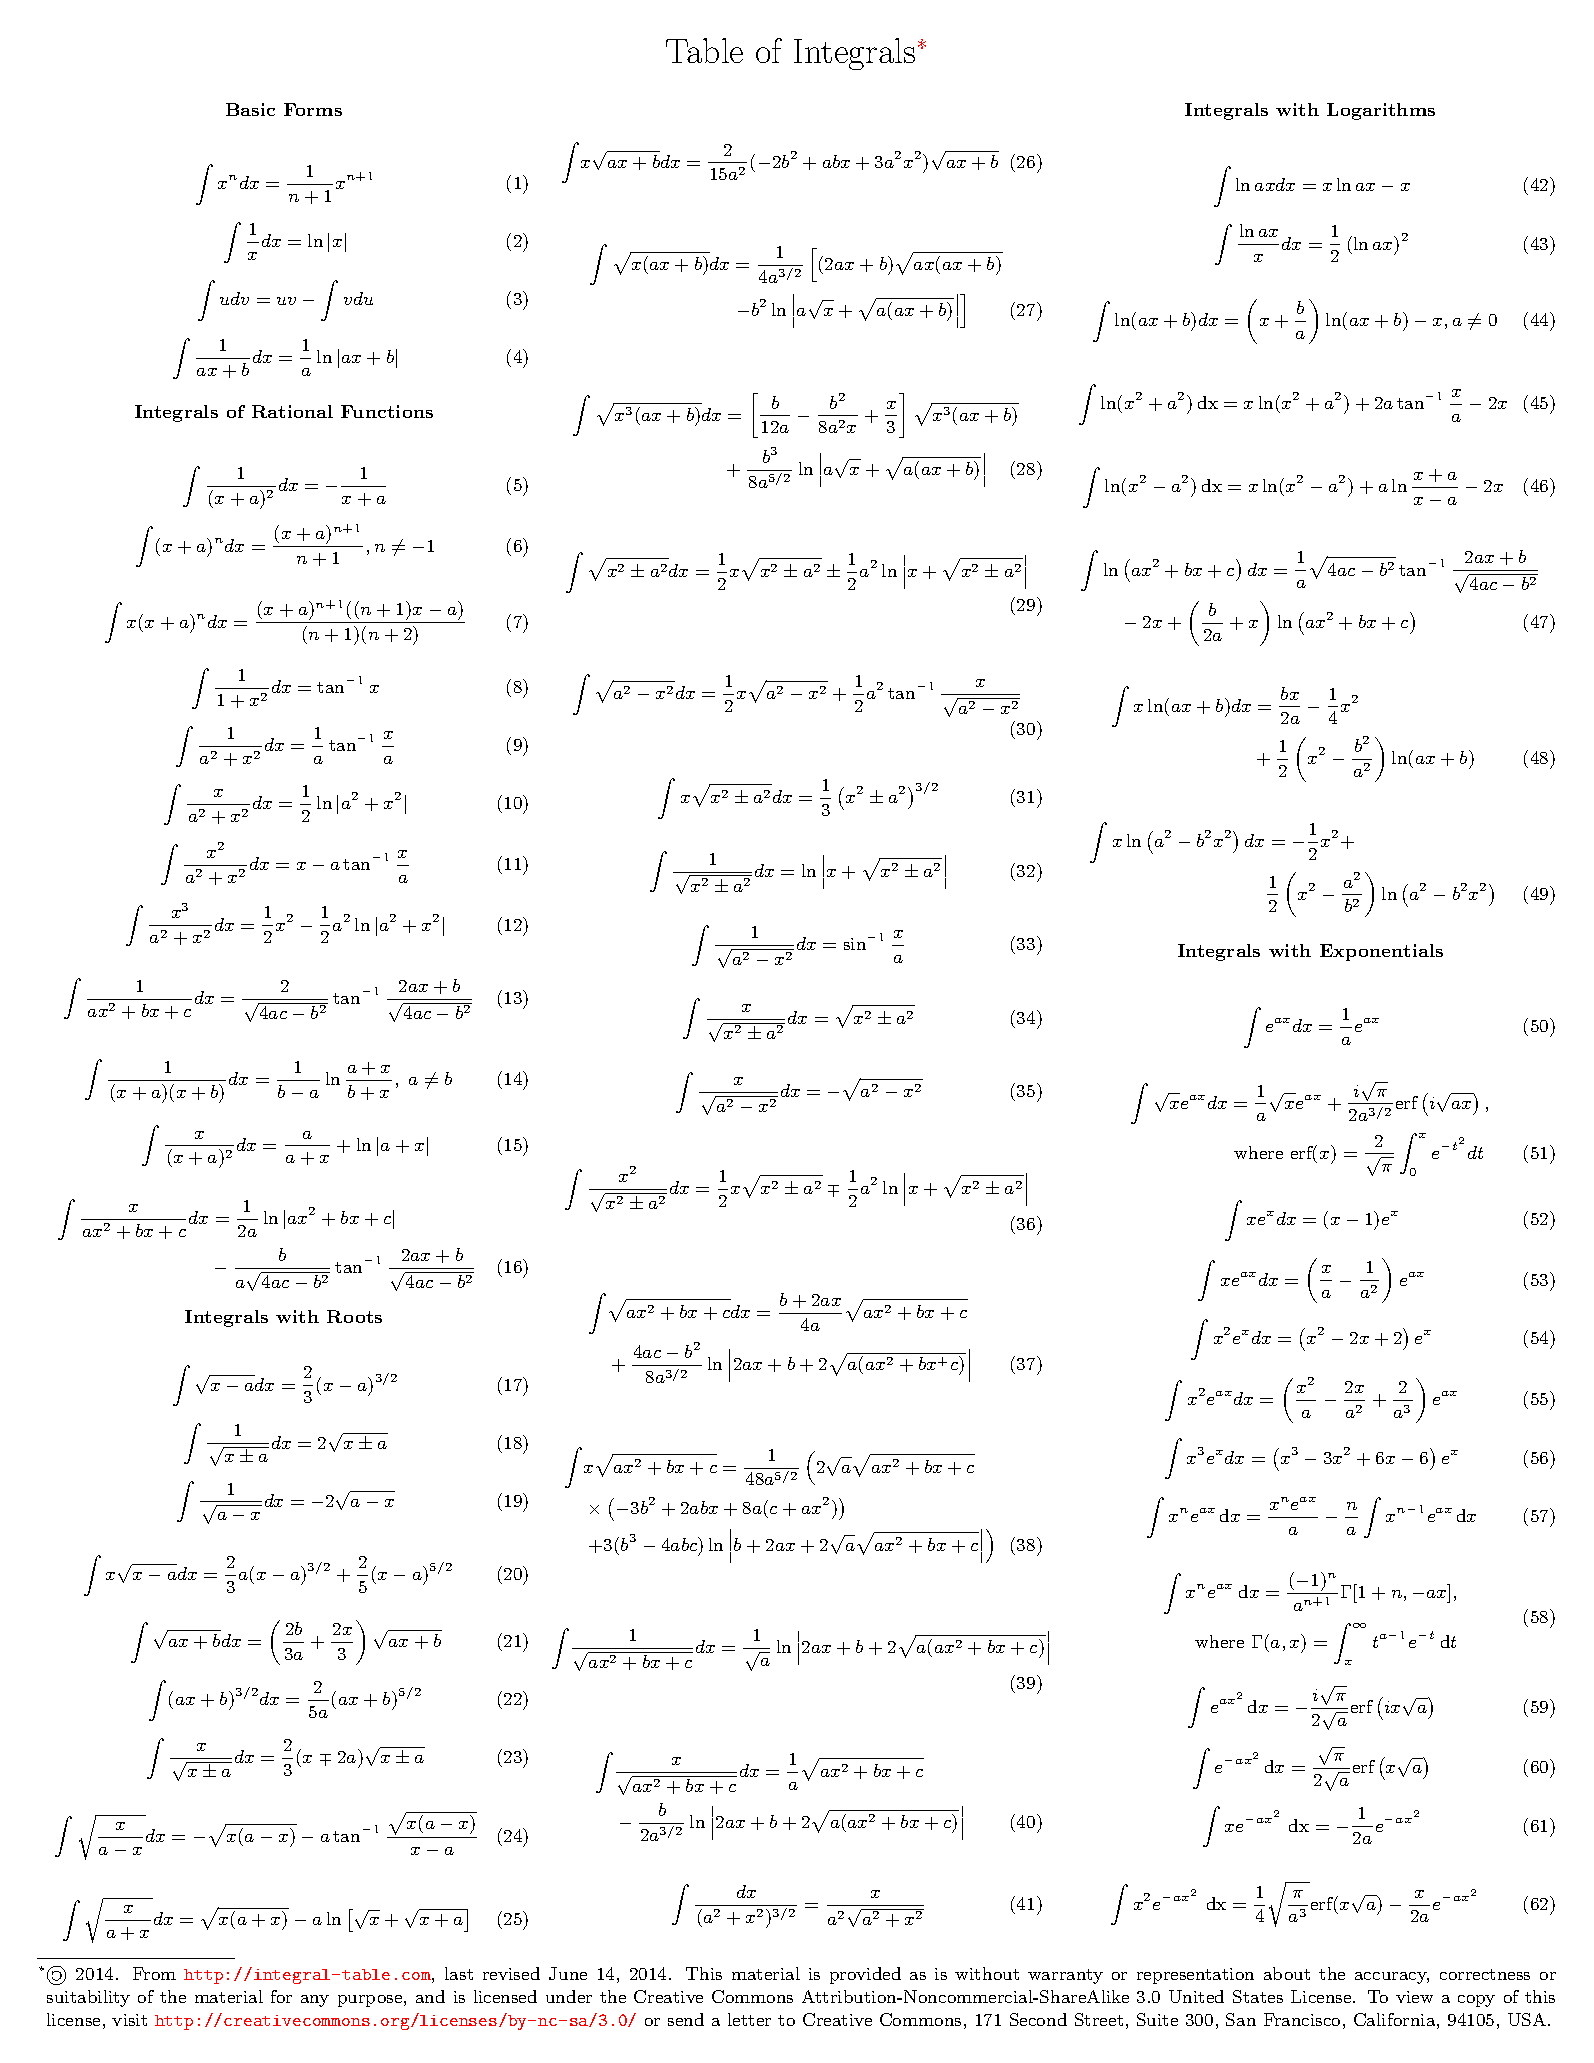
\includepdf[pages=-,pagecommand={\pagestyle{fancy}}]{final/stuff/integralTable.pdf}

\newpage
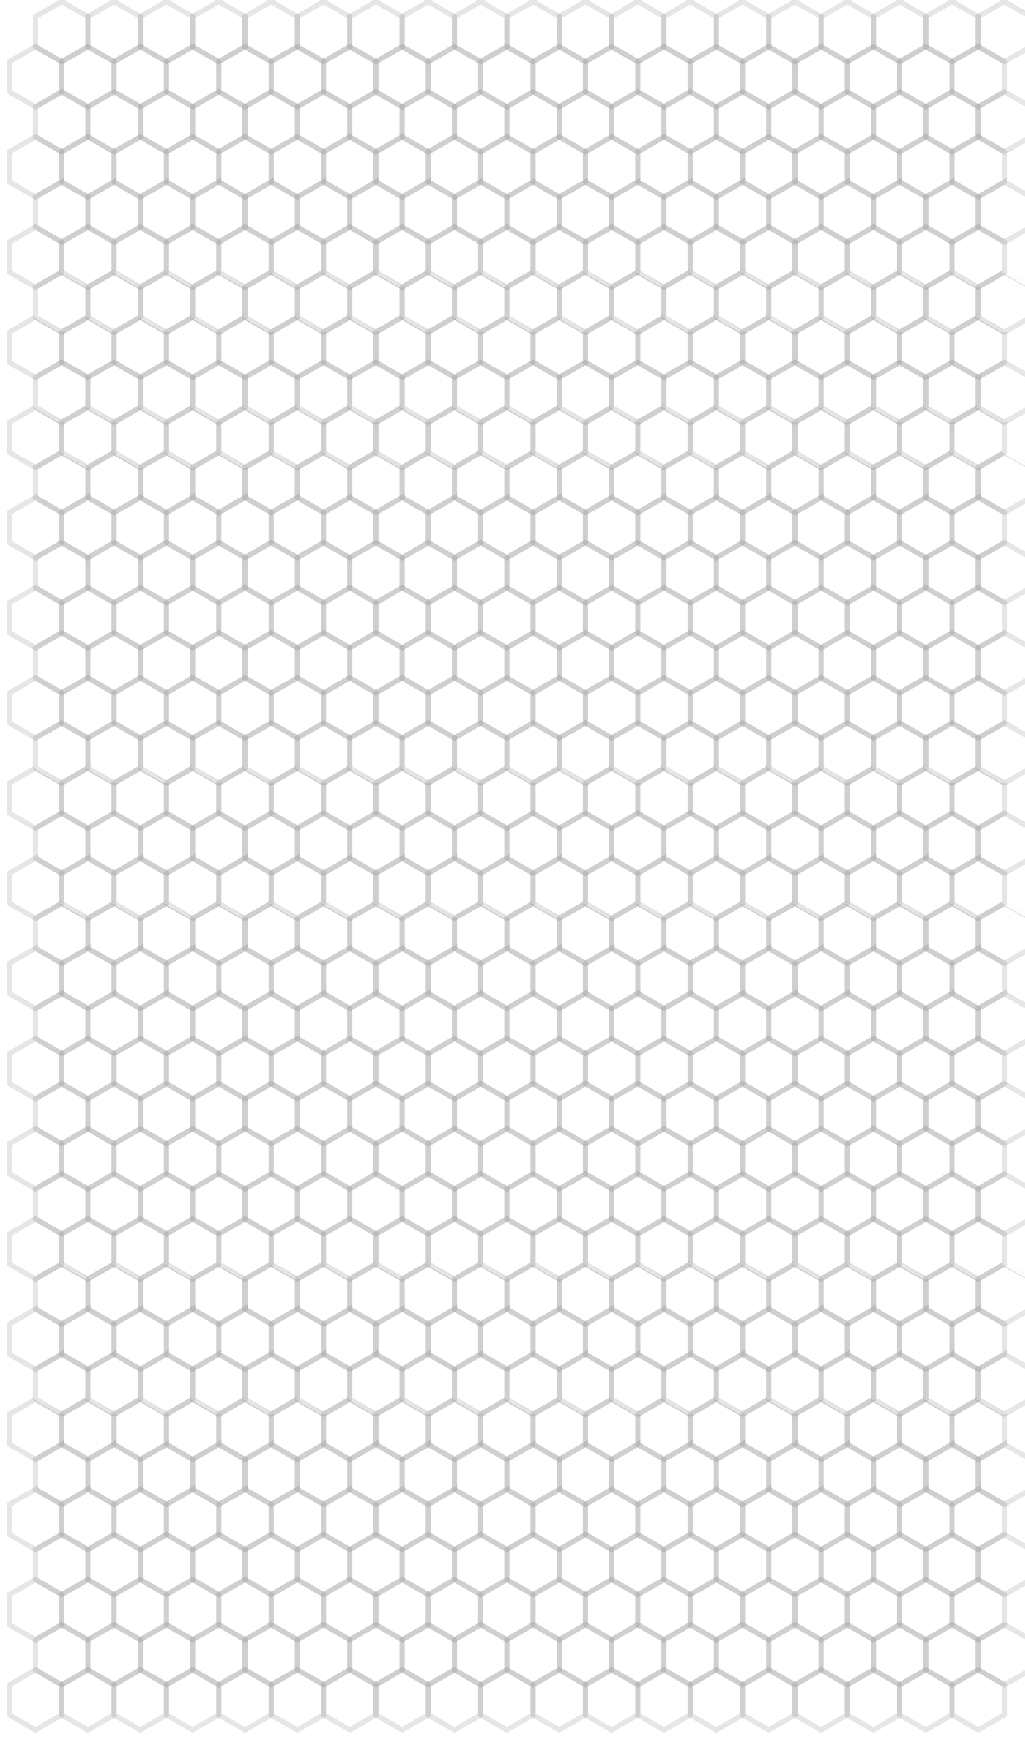
\includepdf[pages=-,pagecommand={\pagestyle{fancy}}]{final/stuff/hexagonal.pdf}
%\newpage
%\twocolumn[
%
\includegraphics{final/stuff/hexagonal.ps}
%]

%\begin{center}
%
\includegraphics{final/stuff/hexagonal.ps}
%\end{center}


%\end{landscape}
\end{document}